\chapter{Speech Fundamentals: Phonetics and Prosody}
\label{StateOfArt}

The purpose of this chapter is to introduce the reader to basic aspects of speech research, the investigation of spoken language. This is, of course, a very wide field covering linguistic, cognitive, and physiological aspects. We will concentrate strictly on the topics relevant to my own proposal: segmental phonemes and supra-segmental prosodic units of language, and two very popular research tools, Praat and Elan.

\section{Elements of spoken language}

In this section, we will first discuss phonemes in spoken language and then turn to prosodic features, which are easily underrated in their importance.

\subsection{Phonemic Segments and Variability}

One essential characteristic of human languages is what has been called "duality of patterning" or "double articulation" \cite{hockett1958course}, \cite{martinet1960elements}: The smallest meaningful units of human speech, such as individual words, consist of sequences of units that themselves have no meaning: the speech sounds or phonemes. For example, the English word \textit{dogs}, consisting of the lexeme \textit{dog} and the suffix morpheme \textit{-s}, is expressed by the sequence of phonemes that can be rendered as /\textipa{dO:gz}/, according to the International Phonetic Alphabet (IPA) \cite{internationalphoneticassociation1999ipa}.

Phonemes can be realized differently by different speakers and in different contexts. They can be realized by different ``allophones'', such as English /p/ as aspirated in [\textipa{p\super{h}In}] \textit{pin} and non-aspirated in [\textipa{spIn}] \textit{spin}, but more importantly, they often have a range of realizations depending on the environment which they occur in \cite{internationalphoneticassociation1999ipa}. For example, the velar stop /k/ is realized more fronted in \textit{kit} than in \textit{cat}. This range of possible realizations is most dramatic with vowels, not only between speakers but also for a single speaker. For example, in a study that investigated both the physiology of production and the acoustic features of vowels, the spread of vowels, characterized by their first and second formants $F_1$ and $F_2$ as illustrated in Figure~\ref{fig:vowelvariation}, was reported. Note the considerable amount of overlap in this reduction of continuous values to discrete categories, which is mostly due to the influence of adjacent phonemes that affect the realization, a phenomenon known as "coarticulation" .

\begin{figure}
    \centering
    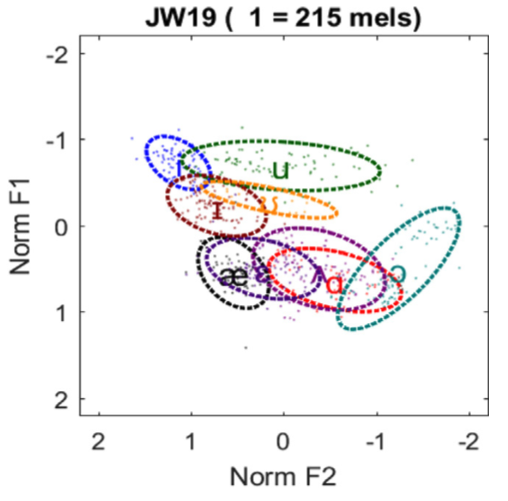
\includegraphics[width=0.5\linewidth]{vowelvariation.png}
    \caption{Realization of vowels by an English speaker, adapted from \cite{whalen2018}.}
    \label{fig:vowelvariation}
\end{figure}

It is a remarkable fact that each language makes use of a small set of phonemes to express a much wider variety of lexical meanings. This set is in the magnitude of about 25 consonants and 8 vowels on average, but shows a considerable variation (e.g. from 6 consonants in the Oceanic language Rotokas and 122 consonants in the San language !Taa, \cite{dryer2013wals,maddieson2013consonant,maddieson2013vowel}). These phonemes distinguish between different meanings (e.g.\ /\textipa{dO:gz}/ vs.\ /\textipa{lO:gz}/ and /\textipa{di:gz}/) and are acquired by children during their first year, before other aspects of language learning develop \cite{kuhl2004early}. The phonemic structure is the ultimate reason why alphabetic writing is possible: The letters, or graphemes, and their order in space in the standard direction of the orthography, correspond in some tighter or looser way to the phonemes and their order in time.

\subsection{Suprasegmentals: Prosody}

In addition to the digital and sequential nature of phonemes, often called ``segments'', spoken language is also characterized by prosody. Prosodic features typically apply to sequences of segments, like syllables, words, syntactic phrases, or whole speech acts, and hence are called ``supra-segmentals''. They also contribute to meaning. Famously, in tone languages they distinguish between different lexemes or grammatical meanings. For example, Mandarin \textit{b\=eizi} 杯子 means `cup, glass', whereas \textit{b\`eizi} 被子 means `quilt, blanket', where the macron (\={}) and grave accent (\`{}) denote high and falling pitch on the first syllable, respectively. In Edo, a West-African language, pitch can distinguish grammatical meanings, as in \textit{ì mà} 'I show' (present, habitual), \textit{ì má} 'I showed' (past tense), and \textit{í mà} 'I am showing' (progressive) \cite{ladefoged1975}. But as we will see below in greater detail, pitch variations are also used in languages like English for tasks like highlighting new or important parts of the message or backgrounding known of given parts, for distinguishing between speech acts like assertions, questions, exclamations, and callings, and for the expression of attitudes and emotions. As recent research shows, this often occurs alongside manual and facial gestures.

The smallest unit in terms of sequences of phonemes that are affected by prosody is the syllable, a sequence of phonemes that follows certain conditions. Syllables consist of an ``onset,'' one or more consonants, followed by a ``rhyme'' that itself consists of a ``nucleus'' and a ``coda.'' For example, /\textipa{dOgz}/ consists of one syllable with onset /d/, rhyme /\textipa{Ogz}/, nucleus /ɔ/, and coda /ɡz/. The syllable is important for prosody because it is one important locus where tones are located. In a stress language like English, words can be distinguished by the location of the stressed syllable, which is determined by the lexical information about the word. An example of this type is /\textipa{"Inv@lId}/ `not valid' and /\textipa{In"v\ae lId}/ `sick or disabled person', where the stressed syllable is indicated by the preceding symbol ˈ, and the differences in the segments are a direct result of the different accent patterns, as the unstressed syllable becomes more centralized and ``weaker.'' There are dozens of minimal pairs denoting nouns and related verbs, such as /\textipa{"prEz@nt}/ `a present' and /\textipa{prI"zEnt}/ `to present', and similarly /\textipa{"EkspOrt}/ and /\textipa{Ik"spOrt}/ `export', /\textipa{"rEb@l}/ and /\textipa{rI"bEl}/ `rebel', and /\textipa{"proUdus}/ and /\textipa{pr@"dus}/ `produce'.

Prosody is also important for complex constructions. For example, we can distinguish between the two meanings of \textit{hot dog} by stress, as /ˈhɑt dɔɡ/ (a bread with a sausage) and /hɑt ˈdɔɡ/ 'a dog that is hot', the first being a compound, and the second, an adjective-noun combination. Prosody can differentiate between different syntactic structures as well, as in [\textit{English} [\textit{history} \textit{teacher}]] /ˈɪŋɡlɪʃ hɪstəri ˌtiːtʃɚ/ and /ˌɪŋɡlɪʃ ˈhɪstəri tiːtʃɚ/ [[\textit{English} \textit{history}] \textit{teacher}], whereˌ indicates a secondary stress. Furthermore, stress can distinguish between different highlighting or focus, which can lead to drastically different interpretations. In the following examples, the sentences are given in standard orthography, for readability, with the word that contains the stressed syllable highlighted.

\begin{itemize}
    \item \textit{\textbf{I} didn't say she stole the money}. (Someone else said it).
    \item \textit{I \textbf{didn't }say she stole the money}. (I deny saying it).
    \item \textit{I didn't \textbf{say} she stole the money.}	(I just implied it).
    \item \textit{I didn't say \textbf{she} stole the money.} (I said someone else stole it.)
    \item \textit{I didn't say she \textbf{stole} the money}. (Maybe she borrowed or found it).
    \item \textit{I didn't say she stole the \textbf{money}.} (I said she stole something else.)
\end{itemize}

Finally, the realization of a stressed syllable by rising or falling prosody provides clues about the sentence type. For example, while English has syntactic means to distinguish between an assertion and a question, as in \textit{I am ready.} in contrast to \textit{Are you ready?}, we can express a question with assertive syntax, as in \textit{You are ready?} Also, a question like \textit{Do you want /tea or \textbackslash coffee?}, with rising and falling accent as indicated by / and \textbackslash, is an alternative question that cannot be answered by \textit{Yes} or \textit{No}, but requests answers like \textit{Coffee, please}. In contrast, the question \textit{Do you want tea or /coffee?}, with one rising accent at the end, is a yes/no question that can be answered with \textit{Yes, coffee} or \textit{No}.


Linguistic research has identified many ways in which prosody is essential for communication. Without question, it plays a crucial role in spoken language. In written language, it is represented only incompletely, if at all, through devices such as punctuation marks and occasionally boldface and underlining. Interestingly, in comics we sometimes find attempts to enliven the presentation by using highlighting and italics as focusing devices, as illustrated in \ref{fig:comics}.

\begin{figure}
    \centering
    
\includegraphics[width=0.95\linewidth]{logicomix.png}
    \caption{Highlighting in writing by boldface and italics in comics. Example: \textit{An epic search for truth} \cite{logicomix}} }
    \label{fig:comics}
\end{figure}


This must suffice to illustrate the extremely important role of prosody in spoken language. But what are the acoustic features in the speech signal that are exploited to indicate what we call "prosody"? The following dimensions are commonly distinguished:

\begin{itemize}
\item Pitch, the fundamental frequency (F0) of the vocal cord, audible over vowels and voiced consonants, like nasals. Measured in cycles per second (hertz), absolute values are speaker-dependent and therefore less important than relative values, such as high and low pitch, or pitch contours such as rising, falling, rise--fall, and fall--rise patterns.
\item Duration, the length of items, in particular syllables, measured in milliseconds. Again, relative values (like having a shorter or longer duration than adjacent syllables) are more important than absolute values.
\item Amplitude, the intensity or sound pressure levels, measured in decibels.  Again, relative values are more relevant than absolute values.
\item Timbre, or phonatory quality, which shows up in different distributions of energy in the frequency rank, and which we will exclude from discussion here.
\item Pauses, often related to breathing, in particular between constituents.
\end{itemize}

There appears to be a fundamental distinction between segments and prosody: As we have seen with \ref{fig:vowelvariation}, the analog variability in the production of segments is reduced to distinct categorical phonemes (here, vowels like /i/, /ɪ/, /u/, /æ/ etc. In prosody, it appears that not only is the encoding done by analog means, but also the things encoded have an analog character. For example, the higher the pitch is raised, or the more the amplitude is increased, the more ``excited'' the speaker sounds. Also, it has been argued that rules that assign stress to the syllables in syntactic phrases do so in a way that varies stress levels indefinites \cite{ChomskyHalle}, e.g. in \textit{bláckbird húnting competítion}, the stressed syllables decrease in their stress level. 

However, there is also evidence that the meanings of prosodic markers identify distinct categories. In particular, a prominent theoretical framework, ToBI (for "tone and break indices") \cite{beckman2006tobi} assumes a limited number of tonal phonemes like L and H for low and high tone that can be combined, e.g. LH for rising, and combinations thereof, and a use of these tonal phonemes as either nuclear accents (marked by *) or accents that indicate boundary levels (marked by \%). There is evidence that, for example, the difference between falling assertion prosody and rising question prosody is perceived categorically \cite{liu2012categorical}, and there are tunes with distinct meanings \cite{Westera2020} There is evidence that, for example, the difference between falling assertion prosody (e.g. \textit{You're coming.}) and rising question prosody (e.g. \textit{You're coming?}) is perceived categorically \cite{liu2012categorical}.

Prosody is often seen as less central to human language than segmental features. But this is a misconception, due to the importance of written language. Pitch, stress, and pauses are not systematically and conventionally expressed in writing, one possible reason being that they are not perceived as categorical like phonemes. Punctuation signs like commas, full stops, and question marks give only vague indications about prosody, and highlighting by capitalization or boldfacing is not obligatory in orthography. Their importance for spoken human language is very evident, and features of prosody have been a major topic in linguistic research (cf. e.g. the articles in \cite{gussenhoven2021oxford}. However, there is less standardization in the description of prosodic phenomena than in the description of segmental phonology.

\section{Tools for investigating spoken language}

After a very cursory overview of the structure of spoken language in segmental and supra-segmental units, we will now turn to the ways how linguistics engage with spoken languages and then will have a look at two essentials tools that are used all over the world and over several disciplines in the research of individual languages. There are alternatives, but these programs have become de facto standards for what they do. We will not mention additional auxiliary programs, such as Audacity [# cite] for purposes like cutting, cleaning, and amplifying recordings.


\subsection{Praat}

Praat is a free, open-source software for speech analysis and synthesis. Developed and maintained by Paul Boersma and David Weenink at the University of Amsterdam around 2000 \cite{boersma2001praat}, it has become a widely used standard tool for speech analysis and synthesis in phonetics, conversation analysis, sociolinguistics, dialectology and field work on endangered languages. Praat is a stable and mature workbench for the analysis, manipulation and synthesis of speech. As illustrated by Figure \ref{fig:praatscreen}, it provides users access to waveforms and spectrograms and allows for the extraction, graphical rendering, and measuring of pitch (F0), amplitude, formants, duration, and intensity. Sound files can be annotated on multiple tiers and in a structured way. \ref{fig:praatscreen} is an example of a Praat screen with amplitude, spectrum, pitch, and various annotation tiers. Data can be exported in various ways for further analysis by statistical programs. Users can access and manipulate sounds with a GUI scripting language. Over the years, many useful scripts and routines have been developed \cite{Styler2022}. Praat has been used as a tool for the transcription of spoken languages, and it offers tools for the precise determination of landmarks and boundaries for vowels and consonants, e.g.\ identifying vowel onset and offset boundaries or measuring voice onset time in stop consonants. One slight disadvantage of Praat is that it is maintained in a somewhat irregular way and does not have strong institutional support.


\begin{figure}
    \centering
    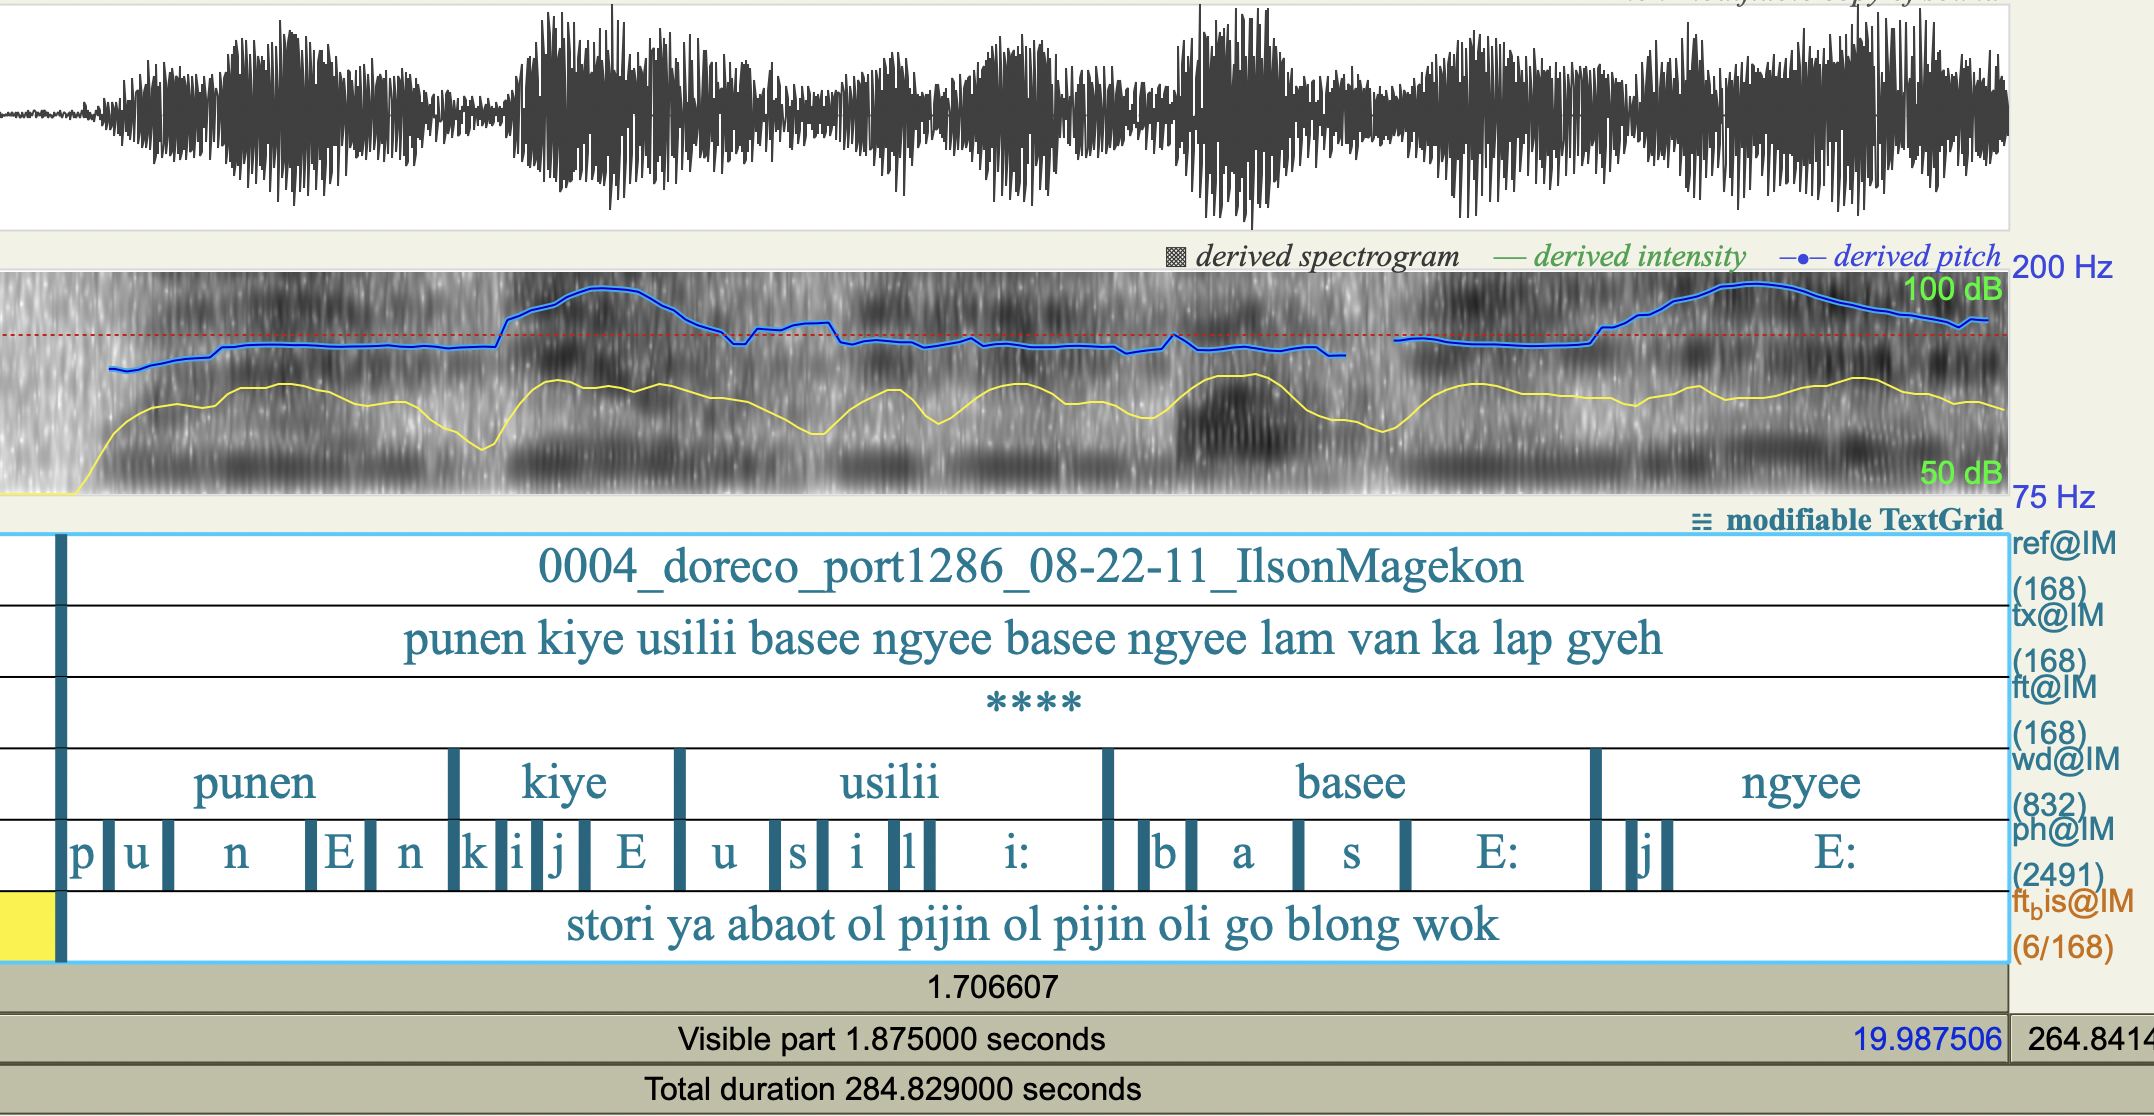
\includegraphics[width=0.95\linewidth]{praatscreen.png}
    \caption{Example of a Praat work screen, from a recording of the language Daakie (Oceanic, Vanuatu), derived from the DoReCo corpus \cite{paschen2020doreco}. From top to bottom: Amplitude, spectrogram with intensity (yellow) and F0 (blue), sentence number and recording identifier, transcription, time-aligned words, time-aligned segments and translation, here to the English-based creole language Bislama.}
    \label{fig:praatscreen}
\end{figure}

One important extension of Praat is Parselmouth, a Python library that provides access to Praat's speech-analysis functions \cite{jadoul2018parselmouth}. Whereas Praat is normally used through its graphical interface or Praat scripting language. Parselmouth allows performing similar functions in Python, such as extracting pitch/F0, intensity, formants, and duration. It can directly access Praat's C/C++ code, so the algorithms and outputs are intended to match Praat itself. Parselmouth is particularly helpful for executing complex workflows in experimental research, such as measuring F0, pitch range, intensity, or formats across many .wav files containing experimental items, and saving the results in a .csv file. Thus, it combines Praat's well-established phonetic algorithms with the broader Python ecosystem.

\subsection{ELAN}

Similar to Praat, ELAN was released in 2000; it was developed and is maintained by the Max-Planck Institute for Psycholinguistics in Nijmegen \cite{sloetjes2008annotation}. The focus is not on the analysis of speech but on the annotation of audiovisual events, particularly communication events. Hence, ELAN allows the work with video files, including multiple video files, that are important for the investigation of gestures, turn-taking, non-verbal communication, as in sign languages, and the interaction of people with their environment. With ELAN, researchers can create a virtually unlimited number of tiers that are can be hierarchically organized. This allows for the annotation of different features of communicative events and for different speakers. ELAN produces XML files of the .eaf type and allows export to more than 20 other formats.  It is highly developed for the extraction of annotation files to other programs, such as spreadsheets, statistics software, language analysis tools, and of course also Praat. It is optimized for the purposes of linguistic field work (in fact, it was used for all research projects of the DOBES project of the Volkswagen Foundation (see \url{https://dobes.mpi.nl/}) and is used in the Endangered Languages Documentation Programme ELDP (see \url{https://www.eldp.net/})). ELAN is used in a wide array of disciplines beyond linguistics, for example in psychology, education, behavioral studies, and animal communication. With the strong and ongoing support of the Max Planck Society, it is continually developed and improved through frequent updates.

The main purpose of ELAN is to simplify and streamline the annotation of audio-visual files. There are different input formats, and tools like identifying segments for repeated listening and slowing down and speeding up recordings. It also allows for the rapid manual partition of recordings into segments that can be analyzed more deeply in subsequent steps, which is particularly important for long audiovisual files that record speech in natural environment. For linguistic annotation, ELAN is optimized for sentences or prosodic phrases, but not for smaller units such as individual words or morphemes. A typical Elan screen is illustrated in Figure \ref{fig:ELANScreen}.

\begin{figure}
    \centering
    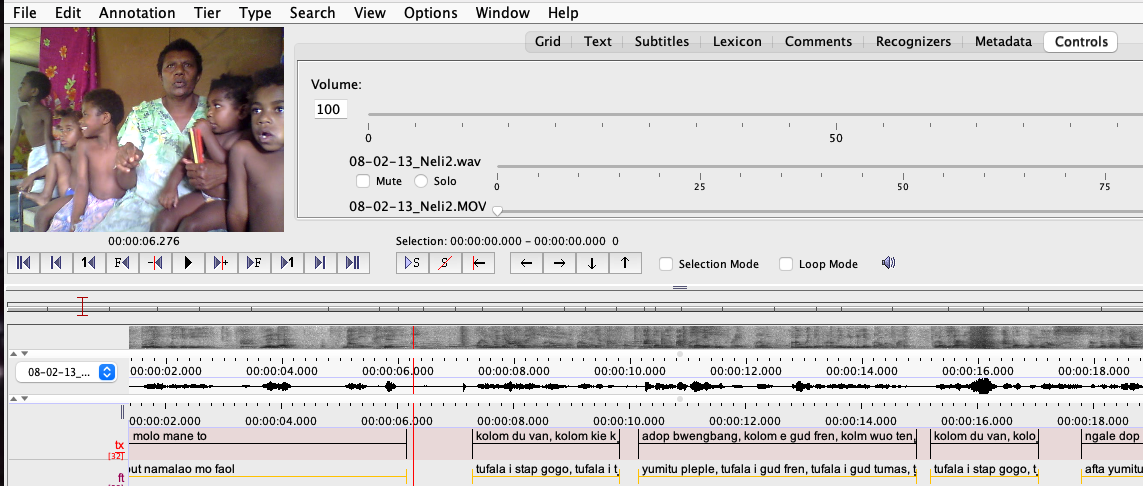
\includegraphics[width=1\linewidth]{DaakieELAN3.png}
    \caption{Cutout from an ELAN screen, with video and audio represented by a spectrum and an amplitude. Annotation tiers are original language (Daakie) and translation into the national language, Bislama.}
    \label{fig:ELANScreen}
\end{figure}


\subsection{Limitations and integration gap}

ELAN does not currently provide tools that assist researchers in the transcription of spoken language beyond showing the amplitude and a rather limited spectrogram. In particular, there is no information about pitch movement (except what is inherent in the small spectrogram), and there is no information about possible phonological segments of the language. Users interested in such more fine-grained analyses are supposed to turn to specialized tools, like Praat. While there is an export function that turns ELAN annotation files to Praat annotation files, a rapid switch from one particular point in an ELAN transcription to Praat and back again is not possible.

The current project, SpeechPrint, aims to improve this situation by providing annotators with helpful information about the segmental and prosodic structure of sound files. For this, it uses automated speech recognition techniques to pre-analyze audio data with respect to prosody and phonemes. This should result in at least two tiers: one for time-aligned phonemes and one for pitch movement; additional tiers for syllable structure or pauses could also be integrated. The annotations in the additional tiers don't have to be accepted at face value by the researcher; they can either serve as a source of helpful information or be corrected and used for further analysis.

It should be explicitly stressed that a careful expert analysis using tools like Praat would provide better, more reliable results than automated techniques can deliver. However, the motivation of this thesis is that such techniques are useful as a support for human annotators. One could argue that human annotators could use existing tools, such as Whisper (see below), anyway. However, linguistic field research is often conducted by researchers who are not trained to use such tools. For example, the Endangered Languages Documentation Project (ELDP) regularly recruits native speakers, or speakers of related languages, as researchers. While these speakers have a genuine insight into their languages, they often lack the training in using sophisticated tools. In such usage scenarios, SpeechPrint can provide some help in the crucial, and often tedious, early step of annotation.

To motivate the feasibility of this goal, we will turn to a brief review of automated speech recognition and the promising tools that have become available and should be relevant to the task at hand.
